\documentclass{article}
\usepackage[latin1]{inputenc}
\usepackage{amsmath}
\usepackage{amssymb}
\usepackage{pgf}
\usepackage{tikz}
\usepackage{verbatim}
\usetikzlibrary{arrows,automata}

\begin{document}

\title{Tools and Algorithms for Deciding Timed Relations}

\author{Mihir Mehta\\
Department of Computer Science and Engineering,\\
Indian Institute of Technology, Delhi.\\
\texttt{cs1090197@cse.iitd.ac.in}
}

\date{December 2012}

\maketitle

\begin{abstract}
This is a report summarising the author's project on their B Tech
Project for the academic year 2012-2013.
\end{abstract}

\section{Objectives}

\begin{itemize}

\item To develop a software toolkit that would enable users to verify
  various timed behavioural equivalences between systems expressed as timed automata.

  \begin{itemize}

  \item To gain an understanding of the theory related to labeled
    transition systems, CCS processes and timed automata by surveying
    relevant literature.

  \item To study existing tools for deciding timed relations.

  \item To implement algorithms for determining timed relations.

  \item To develop the software in a modular way with modules for
    language specification and modules for implementations of utility
    algorithms.

  \end{itemize}

\end{itemize}

\section{CCS processes}

\begin{itemize}
\item A CCS process is an automaton with state and interfaces for
interaction.
\item The interaction is in the form of \emph{actions} over
communication ports known as \emph{channels}.
\item Given a port name $a$ we refer to $a$ as the label for input on the port
  and $\overline{a}$ as the label for the output on the port.
\item \emph{Inaction}: This is the simplest CCS process, denoted by
  $0$. No state transitions or communcation can occur, in other words,
  this represents a deadlock.
\item \emph{Prefixing}: This is the simplest constructor; if $P$ is a
  process and $a$ is a label (input or output) then $a.P$ is also a
  process which can perform the action $a$ in order to become the
  process P. Thus, $\overline{dot}.\overline{dash}.0$ is a CCS process capable of
  transmitting the Morse code letter $A$, and
  $dot.dash.0$ is a process capable of receiving
  it.

\item \emph{Naming}: We can give names to processes using syntax such as \\
$ M \overset{def}{=} dot.dash.0$ \\
$ N \overset{def}{=} \overline{dot}.\overline{dash}.0$ \\
This gives us the ability to define CCS processes recursively, such as
this one:\\
$ Repeater \overset{def}{=} \overline{dot}.\overline{dash}.Repeater$\\
which is a process that continuously repeats the Morse code letter $A$.

\item \emph{Choice}: If $P$ and $Q$ are processes, then $P+Q$ is a
  process as well which has the initial capabilities of both P and
  Q. The deadlock process $0$ is the identity element for this, that is,
  $P+0=P$ is an identity.\\
  Thus, the process $M+N$ could either
  transmit or receive the letter $A$.

\item \emph{Parallel Composition}: If $P$ and $Q$ are
  processes, then $P|Q$ is a process as well in which P and Q may
  proceed independently or communicate via complementary ports.\\
  Thus, the process $M|N$ could proceed with $N$ transmitting the
  letter $A$ to be received by $M$, or they could communicate with
  other processes using the $dot$ and $dash$ ports.

\item \emph{Restriction}: If $P$ is a process and $L$ is a set of
  channel names, then $P/L$ is a process in which the component
  processes of $P$
  are the only processes which can communicate over channels from the
  set $L$.\\
  Thus, $(M|N)/\{dot,dash\}$ would be a process in which $M$ and $N$
  can only communicate with each other.

\item \emph{Relabeling}: If $P$ is a process and $f$ is a function
  from labels to labels, then $P[f]$ is a process where each label
  from the domain of $f$ is replaced by its image under $f$. One
  application of relabelling is the idea of \emph{generic} processes:
  By relabelling the generic ports of such a process with specific
  port names, one can generate specific processes.

\end{itemize}

It is evident that each CCS process can be replaced by a labeled
transition system (LTS) with equivalent behaviour, therefore we will,
in the rest of this discussion, freely use the properties of LTS when
describing those of CCS.

\section{Equivalences on CCS}

\subsection{Trace equivalence}
  \begin{itemize}

  \item A \emph{trace} of an LTS is a sequence of actions
    that the LTS can perform.

nn  \item For an LTS $P$, the set $Traces(P)$ represents the set of all
    possible traces of $P$.
  \item Trace equivalence is said to exist between two LTS $P$ and $Q$
    when $Traces(P) = Traces(Q)$.
  \item However, this notion proves to have a significant limitation
    in the case of CCS processes: Two CCS processes can have trace equivalence
    between their corresponding LTS and yet behave differently in
    terms of when they deadlock while interacting with a third CCS
    process.
  \item Consider, for instance, the machines \\
    $(dot.dash.(\overline{dot}+\overline{dot}.\overline{dot})).0$\\
    and\\
    $(dot.dash.\overline{dot})+(dot.dash.\overline{dot}.\overline{dot})$\\
    Both of these have the same trace set, which consists of accepting
    the Morse letter $A$ and transmitting either $E$ or $I$. However, when
    interacting with a third process that transmits $A$ and accepts
    $E$, \\
    $\overline{dot}.\overline{dash}.dot$\\
    it is evident that the second process may have a deadlock while
    the first cannot.
  \end{itemize}

\subsection{Strong bisimilarity}
  \begin{itemize}
  \item \emph{Strong bisimulation}: A binary relation $R$ is a \textit{strong
    bisimulation} if and only if, for all $(s_1, s_2)$ $\epsilon$ $R$ and $a$ $\epsilon$ $Act .$\\
    $\forall s_1' (s_1 \xrightarrow{a} s_1' \Rightarrow \exists s_2'
    . (s_2 \xrightarrow{a} s_2' \wedge (s_1', s_2')$ $\epsilon$ $R ) )
    \wedge $ \\
    $\forall s_2' (s_2 \xrightarrow{a} s_2' \Rightarrow \exists s_1'
    . (s_1 \xrightarrow{a} s_1' \wedge (s_1', s_2')$ $\epsilon$ $R ) )$
  \item \emph{Strong bisimilarity}: It can be shown that the union of
    all strong bisimulations
    over the set of states is a strong bisimulation. This binary
    relation is called \textit{strong bisimilarity}, denoted by $\sim$.
  \item This mitigates one of the failings of trace equivalence as an
    equivalence relation: strong bisimilarity between two CCS
    processes ensures identical deadlock behaviour while interacting
    with a third CCS process.
  \item However, another limitation soon becomes apparent: if two CCS
    processes are to be strongly bisimilar, they must coincide even on
    the number and position of $\tau$ transitions in their
    traces. This is contrary to the semantics of CCS processes, as
    a $\tau$ transition is supposed to be private to a process and
    invisible to all other processes in its environment.

  \end{itemize}

\subsection{Weak bisimilarity}

  \begin{itemize}
  \item \emph{Weak bisimulation}: A binary relation $R$ is a \textit{weak
    bisimulation} if and only if, for all $(s_1, s_2)$ $\epsilon$ $R$ and
    $a$ $\epsilon$ $Act .$\\
    $\forall s_1' (s_1 \xrightarrow{a} s_1' \Rightarrow \exists s_2'
    . (s_2 \overset{a}{\Rightarrow} s_2' \wedge (s_1', s_2')$ $\epsilon$ $R ) )
    \wedge $ \\
    $\forall s_2' (s_2 \xrightarrow{a} s_2' \Rightarrow \exists s_1'
    . (s_1 \overset{a}{\Rightarrow} s_1' \wedge (s_1', s_2')$ $\epsilon$ $R ) )$
  \item It can be shown that the union of all weak bisimulations
    over the set of states is a weak bisimulation. This binary
    relation is called \textit{weak bisimilarity}, denoted by $\approx$.
  \item Better suited to CCS processes,
    as it ignores $\tau$ transitions, thus disregarding hidden
    behaviour within a process.
  \end{itemize}

\subsection{Kanellakis and Smolka's algorithm}

  \begin{itemize}
  \item This is a naive algorithm for determining the bisimilarity
    relation for the set of processes in a labelled transition system.
  \item This relies on the notion of a splitter.
  \item Let $\pi = \{ B_0, ..., B_k \}, k \ge 0$ be a partition of the
    set of states $Pr$ in a labeled transition system.
  \item A splitter for a block $B_i$ $\epsilon$ $\pi$ is a block $B_j$
    $\epsilon$ $\pi$ such that for some action $a$ $\epsilon$ $Act$, some
    states in $B_i$ have $a$-labelled transitions whose targets lie in
    $B_j$ while other states in $B_i$ do not.
  \item This suggests a refinement of $\pi$: replace block $B_i$ with
    \\
    $B_i^1 = B_i \cap T_a^{-1}[B_j] $ \\
    $B_i^2 = B_i - B_i^1 $
  \item Refinements of this kind constitute the steps of this
    algorithm.
  \item The time complexity of this algorithm is $O(mn)$, since there
    can be at most n iterations, and all m edges are scanned in each iteration.
  \end{itemize}

\subsection{Fernandez' algorithm}

  \begin{itemize}
  \item This is a more efficient algorithm for determining bisimilarity (O(m log n)).
  \item This relies on the technique of three-way splitting introduced
    by Paige and Tarjan.
  \item Splitters can now be 'simple' or 'compound'.
  \item Stability: A partition $\pi$ is said to be stable with respect to a
    compound block S if S is not a splitter for any block in $\pi$ for
    any action.
  \item For a compound block S, having a constituent simple block B
    satisfying $n(B) \le 0.5*n(S)$, and with respect to which $\pi$ is
    stable, we can split a block $B_i$ on an action $a$ as follows:\\
    $B_i^1 = (B_i \cap T_a^{-1}[B]) - T_a^{-1}[S-B]$ \\
    $B_i^2 = (B_i \cap T_a^{-1}[S-B]) - T_a^{-1}[B]$ \\
    $B_i^3 = B_i \cap T_a^{-1}[B] \cap T_a^{-1}[S-B]$ \\
  \end{itemize}

  \section{Timed automata}

  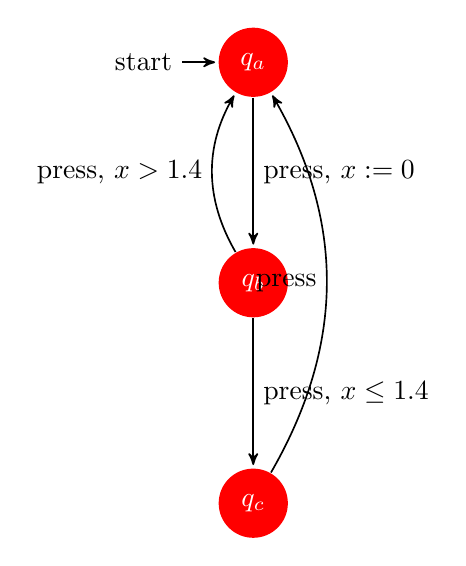
\begin{tikzpicture}[->,>=stealth',shorten >=1pt,auto,node
      distance=2.8cm,
      semithick]
    \tikzstyle{every state}=[fill=red,draw=none,text=white]

    \node[initial,state] (A)                    {$q_a$};
    \node[state]         (B) [below of=A] {$q_b$};
    \node[state]         (C) [below of=B] {$q_c$};
    
    \path (A) edge              node {press, $x:=0$}    (B)
    (B) edge [bend left] node {press, $x > 1.4$}        (A)
    edge              node {press, $x \le 1.4$}         (C)
    (C) edge [bend right] node {press}                  (A);
  \end{tikzpicture}
  
  Timed automaton representing a light bulb with two
  brightness settings, example taken from \textit{Reactive Systems}.

  \begin{itemize}
  \item Formally, a timed automaton over a finite set of clocks $C$
    and a finite set of actions $Act$ is a 4-tuple $(L, l_{0}, E, I)$.
  \item $L$ is a finite set of locations.
  \item $l_{0}$ is the initial location.
  \item $E \subseteq L \times B(C) \times Act \times 2^{C} \times L$
    is a finite set of edges.
  \item $I: L \rightarrow B(C)$ assigns invariants to each edge
    location.
  \item $B(C)$ is the set of clock constraints over C. An element of $B(C)$
    can be an equality, a slack inequality, or a strict inequality on
    $v(x)$ for some $x$ $\epsilon$ $C$, or
    an AND combination of such constraints.
  \item The state of the automaton at any particular instant is given
    by the ordered pair $(l, v)$ which gives the location and assigns
    a value to each clock. 
  \item A transition is either a delay transition where the automaton
    stays at the same location while advancing each clock by the same
    time delay, or an action transition where the automaton performs a
    state change while resetting some of its clocks.
  \end{itemize}
  
  \section{Equivalences on Timed Automata}

  \subsection{Timed bisimilarity}
  
  \begin{itemize}
  \item \emph{Timed bisimulation}: A binary relation $R$ is a timed
    bisimulation if and only if, for all $(s_1, s_2)$ $\epsilon$ $R$ , $a$ $\epsilon$ $Act $, $d$ $\epsilon$ $R_{\ge 0}$\\
    $\forall s_1' (s_1 \xrightarrow{a} s_1' \Rightarrow \exists s_2'
    . (s_2 \xrightarrow{a} s_2' \wedge (s_1', s_2')$ $\epsilon$ $R ) )
    \wedge $ \\
    $\forall s_2' (s_2 \xrightarrow{a} s_2' \Rightarrow \exists s_1'
    . (s_1 \xrightarrow{a} s_1' \wedge (s_1', s_2')$ $\epsilon$ $R ) ) \wedge $ \\
    $\forall s_1' (s_1 \xrightarrow{d} s_1' \Rightarrow \exists s_2'
    . (s_2 \xrightarrow{d} s_2' \wedge (s_1', s_2')$ $\epsilon$ $R ) )
    \wedge $ \\
    $\forall s_2' (s_2 \xrightarrow{d} s_2' \Rightarrow \exists s_1'
    . (s_1 \xrightarrow{d} s_1' \wedge (s_1', s_2')$ $\epsilon$ $R ) ) $ \\
    
  \item It can be shown that the union of all timed bisimulations
    over the set of (location, valuation) pairs is a timed bisimulation. This binary
    relation is called \textit{timed bisimilarity}, denoted by $\sim$.
  \end{itemize}
  
  \subsection{Time abstracted bisimilarity}
  
  \begin{itemize}
    
  \item \emph{Time abstracted bisimulation}: A binary relation $R$ is
    a time abstracted
    bisimulation if and only if, for all $(s_1, s_2) \epsilon R$ , $a \epsilon Act $, $d \epsilon R_{\ge 0}$\\
    $\forall s_1' (s_1 \xrightarrow{a} s_1' \Rightarrow \exists s_2'
    . (s_2 \xrightarrow{a} s_2' \wedge (s_1', s_2')$ $\epsilon$ $R ) )
    \wedge $ \\
    $\forall s_2' (s_2 \xrightarrow{a} s_2' \Rightarrow \exists s_1'
    . (s_1 \xrightarrow{a} s_1' \wedge (s_1', s_2')$ $\epsilon$ $R ) ) \wedge $ \\
    $\forall s_1' (s_1 \xrightarrow{d} s_1' \Rightarrow \exists (s_2',
    d')
    . (s_2 \xrightarrow{d} s_2' \wedge (s_1', s_2')$ $\epsilon$ $R ) )
    \wedge $ \\
    $\forall s_2' (s_2 \xrightarrow{d} s_2' \Rightarrow \exists (s_1', d')
    . (s_1 \xrightarrow{d} s_1' \wedge (s_1', s_2')$ $\epsilon$ $R ) ) $ \\

  \item It can be shown that the union of all time abstracted bisimulations
    over the set of (location, valuation) pairs is a time abstracted bisimulation. This binary
    relation is called \textit{time abstracted bisimilarity}, denoted by $\sim_u$.
    

\end{itemize}

\subsection{Regions and region graphs}

One problem with the notion of valuations is that since they map
clocks to real values, it can be difficult to design algorithms for
determining properties such as
reachability. However, by introducing the notion of equivalence
between two valuations in the context of a timed automaton, we can
divide the uncountably infinite set of valuations into a finite number
of equivalence classes (called regions) which allows us to derive some
useful notions.

\subsubsection{Equivalence of valuations}
Two valuations $v$ and $v'$ of
a timed automaton are said to be equivalent ($v \equiv v'$) if and
only if:
\begin{itemize}
\item For each $x$ $\epsilon$ $C$, either both $v(x)$ and $v'(x)$ are
  greater than $c_x$ or $\lfloor v(x) \rfloor = \lfloor v'(x)
  \rfloor$
\item For each $x$ $\epsilon$ $C$ such that $v(x) \le c_x$,
  $frac(v(x))=0$ if and only if $frac(v'(x))=0$.
\item For all $x$,$y$ $\epsilon$ $C$ such that $v(x) \le c_x$ and $v(y)
  \le c_y$, we have $frac(v(x)) \le frac(v(y))$ if and only if
  $frac(v'(x)) \le frac(v'(y))$.
\end{itemize}

Under this notion of equivalence, an equivalence class is known
as a \emph{region}. The equivalence class containing a valuation $v$
is denoted by $[v]_{\equiv}$.

\subsubsection{Region graph}
With these definitions, we can define the
region graph of a timed automaton as a LTS representation of the
automaton where the action transitions are labelled with the same
actions and the delay self-transitions are labelled with
$\varepsilon$.
Formally, the region graph of a timed automaton $A$ with clock set $C$
and action set $Act$ is an LTS\\
$T_r(A) = (Proc,Act \cup \{\varepsilon\}, \{\xrightarrow{a}|a \epsilon
Act \cup \{\varepsilon\}\})$\\
where $Proc = \{(l, [v]_{\equiv}) | l$ $\epsilon$ $L, v: C \rightarrow
R_{\ge 0}\}$ (these states are called symbolic states)\\
The transitions are defined as follows:
\begin{itemize}
\item For each $a \epsilon A$, $(l, [v]_{\equiv})
  \overset{a}{\Rightarrow} (l', [v']_{\equiv})$ iff $(l,v)
  \overset{a}{\rightarrow} (l', v')$
\item $(l, [v]_{\equiv}) \xrightarrow{a} (l, [v']_{\equiv})$ if
  for some $d$ $\epsilon$ $R_{\ge 0}$, $(l, v) \xrightarrow{d} (l,
  v')$
\end{itemize}

\subsection{Zones and reachability graphs}

Though the region graph provides some useful results about properties
such as reachablility, time
abstracted bisimilarity and so on, its state space can grow very fast as a
function of the number of clocks (the upper bound on the number of
states happens to be exponential in the number of clocks). Using
zones, we can represent the state space of a timed automaton in a more
compact way.

\subsubsection{Extended clock constraints}
These are described by the  grammar\\
$g :: = x \bowtie n | x - y \bowtie n | g_1 \wedge g_2$\\
where\\
$n$ $\epsilon$ $\mathbb{N}$\\
and\\
$\bowtie$ represents any one of the equality, slack inequality and
strict inequality symbols.\\
The set of extended clock constraints is denoted by $B^+(C)$
\subsubsection{Zones}
A zone is a set of valuations represented by an
extended clock constraint.\\
$Z = \{v|v$ $\epsilon$ $g_Z\}$\\
where $g_Z$ represents the defining constraint of $Z$.
\subsubsection{Symbolic state}
For a timed automaton $A$, a symbolic
state is an ordered pair of a location and a zone, that is, $(l,
Z)$.
\subsubsection{Reachability graph}
The reachability graph of a timed
automaton is a directed graph in which the nodes are symbolic states
and the edges are given by the \emph{reachability relation}:
\begin{itemize}
\item $(l,Z')$ is reachable from $(l,Z)$ if there exists a
  valuation belonging $Z'$ which can be obtained
  from Z by applying a time delay which does not violate the
  invariant at $l$.

\item $(l', Z')$ is reachable from $(l, Z)$ if $l$ has an action
  transition to $l'$ and there exists a valuation in $Z'$ which
  violates neither the guard of the
  transition nor the invariant at $l'$.
\end{itemize}

\section{Code written so far}

\subsection{Fernandez' algorithm}

We implemented Fernandez' algorithm in Ocaml to be used as a module in
further applications.

\subsection{Lexical analyser and Parser}

Using a grammar very similar to that employed by the research tool Minim (Stavros
Tripakis et al), we implemented an Ocaml program to parse a timed
automaton from an input file.

The grammar specification we used generates a representation of the
timed automaton which is similar to an adjacency list representation
of a labelled graph.

Here is an example to illustrate the grammar for timed automata that
we are using:

\begin{verbatim}

#states 5
#trans 6
#clocks 2
X3 X5

state: 0
invar: X3 < 5
trans:
X5 >= 7 => RESET { X3 }; goto 1

state: 1
invar: X7 >= 9 and X8 <= 10
trans:
X5 >= 7 => RESET { X3 }; goto 2

state: 2
invar: TRUE
trans:
X5 >= 7 => RESET { X3 }; goto 3

state: 3
invar: TRUE
trans:
X5 >= 7 => RESET { X3 }; goto 4

state: 4
invar: TRUE
trans:
X5 >= 7 => RESET { X3 }; goto 0


\end{verbatim}

\section{References}

\begin{itemize}
\item Reactive Systems: Modeling, Specification and Verification -
  Luca Aceto, Anna Ingolfsdottir, Kim Larsen, Jiri Srba.
\end{itemize}

\end{document}
